\documentclass[1p]{elsarticle_modified}
%\bibliographystyle{elsarticle-num}

%\usepackage[colorlinks]{hyperref}
%\usepackage{abbrmath_seonhwa} %\Abb, \Ascr, \Acal ,\Abf, \Afrak
\usepackage{amsfonts}
\usepackage{amssymb}
\usepackage{amsmath}
\usepackage{amsthm}
\usepackage{scalefnt}
\usepackage{amsbsy}
\usepackage{kotex}
\usepackage{caption}
\usepackage{subfig}
\usepackage{color}
\usepackage{graphicx}
\usepackage{xcolor} %% white, black, red, green, blue, cyan, magenta, yellow
\usepackage{float}
\usepackage{setspace}
\usepackage{hyperref}

\usepackage{tikz}
\usetikzlibrary{arrows}

\usepackage{multirow}
\usepackage{array} % fixed length table
\usepackage{hhline}

%%%%%%%%%%%%%%%%%%%%%
\makeatletter
\renewcommand*\env@matrix[1][\arraystretch]{%
	\edef\arraystretch{#1}%
	\hskip -\arraycolsep
	\let\@ifnextchar\new@ifnextchar
	\array{*\c@MaxMatrixCols c}}
\makeatother %https://tex.stackexchange.com/questions/14071/how-can-i-increase-the-line-spacing-in-a-matrix
%%%%%%%%%%%%%%%

\usepackage[normalem]{ulem}

\newcommand{\msout}[1]{\ifmmode\text{\sout{\ensuremath{#1}}}\else\sout{#1}\fi}
%SOURCE: \msout is \stkout macro in https://tex.stackexchange.com/questions/20609/strikeout-in-math-mode

\newcommand{\cancel}[1]{
	\ifmmode
	{\color{red}\msout{#1}}
	\else
	{\color{red}\sout{#1}}
	\fi
}

\newcommand{\add}[1]{
	{\color{blue}\uwave{#1}}
}

\newcommand{\replace}[2]{
	\ifmmode
	{\color{red}\msout{#1}}{\color{blue}\uwave{#2}}
	\else
	{\color{red}\sout{#1}}{\color{blue}\uwave{#2}}
	\fi
}

\newcommand{\Sol}{\mathcal{S}} %segment
\newcommand{\D}{D} %diagram
\newcommand{\A}{\mathcal{A}} %arc


%%%%%%%%%%%%%%%%%%%%%%%%%%%%%5 test

\def\sl{\operatorname{\textup{SL}}(2,\Cbb)}
\def\psl{\operatorname{\textup{PSL}}(2,\Cbb)}
\def\quan{\mkern 1mu \triangleright \mkern 1mu}

\theoremstyle{definition}
\newtheorem{thm}{Theorem}[section]
\newtheorem{prop}[thm]{Proposition}
\newtheorem{lem}[thm]{Lemma}
\newtheorem{ques}[thm]{Question}
\newtheorem{cor}[thm]{Corollary}
\newtheorem{defn}[thm]{Definition}
\newtheorem{exam}[thm]{Example}
\newtheorem{rmk}[thm]{Remark}
\newtheorem{alg}[thm]{Algorithm}

\newcommand{\I}{\sqrt{-1}}
\begin{document}

%\begin{frontmatter}
%
%\title{Boundary parabolic representations of knots up to 8 crossings}
%
%%% Group authors per affiliation:
%\author{Yunhi Cho} 
%\address{Department of Mathematics, University of Seoul, Seoul, Korea}
%\ead{yhcho@uos.ac.kr}
%
%
%\author{Seonhwa Kim} %\fnref{s_kim}}
%\address{Center for Geometry and Physics, Institute for Basic Science, Pohang, 37673, Korea}
%\ead{ryeona17@ibs.re.kr}
%
%\author{Hyuk Kim}
%\address{Department of Mathematical Sciences, Seoul National University, Seoul 08826, Korea}
%\ead{hyukkim@snu.ac.kr}
%
%\author{Seokbeom Yoon}
%\address{Department of Mathematical Sciences, Seoul National University, Seoul, 08826,  Korea}
%\ead{sbyoon15@snu.ac.kr}
%
%\begin{abstract}
%We find all boundary parabolic representation of knots up to 8 crossings.
%
%\end{abstract}
%\begin{keyword}
%    \MSC[2010] 57M25 
%\end{keyword}
%
%\end{frontmatter}

%\linenumbers
%\tableofcontents
%
\newcommand\colored[1]{\textcolor{white}{\rule[-0.35ex]{0.8em}{1.4ex}}\kern-0.8em\color{red} #1}%
%\newcommand\colored[1]{\textcolor{white}{ #1}\kern-2.17ex	\textcolor{white}{ #1}\kern-1.81ex	\textcolor{white}{ #1}\kern-2.15ex\color{red}#1	}

{\Large $\underline{12n_{0494}~(K12n_{0494})}$}

\setlength{\tabcolsep}{10pt}
\renewcommand{\arraystretch}{1.6}
\vspace{1cm}\begin{tabular}{m{100pt}>{\centering\arraybackslash}m{274pt}}
\multirow{5}{120pt}{
	\centering
	\includegraphics[width=112pt]{../../../GIT/diagram.site/Diagrams/png/2583_12n_0494.png}\\
\ \ \ A knot diagram\footnotemark}&
\allowdisplaybreaks
\textbf{Linearized knot diagam} \\
\cline{2-2}
 &
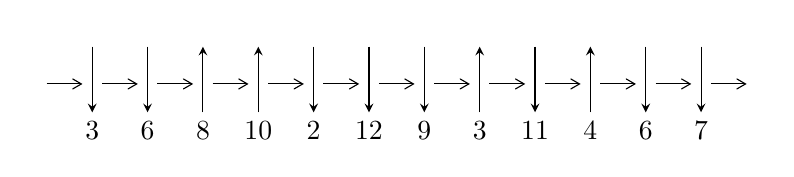
\begin{tikzpicture}[x=20pt, y=17pt]
	% nodes
	\node (C0) at (0, 0) {};
	\node (C1) at (1, 0) {};
	\node (C1U) at (1, +1) {};
	\node (C1D) at (1, -1) {3};

	\node (C2) at (2, 0) {};
	\node (C2U) at (2, +1) {};
	\node (C2D) at (2, -1) {6};

	\node (C3) at (3, 0) {};
	\node (C3U) at (3, +1) {};
	\node (C3D) at (3, -1) {8};

	\node (C4) at (4, 0) {};
	\node (C4U) at (4, +1) {};
	\node (C4D) at (4, -1) {10};

	\node (C5) at (5, 0) {};
	\node (C5U) at (5, +1) {};
	\node (C5D) at (5, -1) {2};

	\node (C6) at (6, 0) {};
	\node (C6U) at (6, +1) {};
	\node (C6D) at (6, -1) {12};

	\node (C7) at (7, 0) {};
	\node (C7U) at (7, +1) {};
	\node (C7D) at (7, -1) {9};

	\node (C8) at (8, 0) {};
	\node (C8U) at (8, +1) {};
	\node (C8D) at (8, -1) {3};

	\node (C9) at (9, 0) {};
	\node (C9U) at (9, +1) {};
	\node (C9D) at (9, -1) {11};

	\node (C10) at (10, 0) {};
	\node (C10U) at (10, +1) {};
	\node (C10D) at (10, -1) {4};

	\node (C11) at (11, 0) {};
	\node (C11U) at (11, +1) {};
	\node (C11D) at (11, -1) {6};

	\node (C12) at (12, 0) {};
	\node (C12U) at (12, +1) {};
	\node (C12D) at (12, -1) {7};
	\node (C13) at (13, 0) {};

	% arrows
	\draw[->,>={angle 60}]
	(C0) edge (C1) (C1) edge (C2) (C2) edge (C3) (C3) edge (C4) (C4) edge (C5) (C5) edge (C6) (C6) edge (C7) (C7) edge (C8) (C8) edge (C9) (C9) edge (C10) (C10) edge (C11) (C11) edge (C12) (C12) edge (C13) ;	\draw[->,>=stealth]
	(C1U) edge (C1D) (C2U) edge (C2D) (C3D) edge (C3U) (C4D) edge (C4U) (C5U) edge (C5D) (C6U) edge (C6D) (C7U) edge (C7D) (C8D) edge (C8U) (C9U) edge (C9D) (C10D) edge (C10U) (C11U) edge (C11D) (C12U) edge (C12D) ;
	\end{tikzpicture} \\
\hhline{~~} \\& 
\textbf{Solving Sequence} \\ \cline{2-2} 
 &
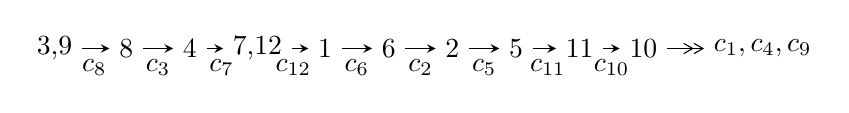
\begin{tikzpicture}[x=23pt, y=7pt]
	% node
	\node (A0) at (-1/8, 0) {3,9};
	\node (A1) at (1, 0) {8};
	\node (A2) at (2, 0) {4};
	\node (A3) at (49/16, 0) {7,12};
	\node (A4) at (33/8, 0) {1};
	\node (A5) at (41/8, 0) {6};
	\node (A6) at (49/8, 0) {2};
	\node (A7) at (57/8, 0) {5};
	\node (A8) at (65/8, 0) {11};
	\node (A9) at (73/8, 0) {10};
	\node (C1) at (1/2, -1) {$c_{8}$};
	\node (C2) at (3/2, -1) {$c_{3}$};
	\node (C3) at (5/2, -1) {$c_{7}$};
	\node (C4) at (29/8, -1) {$c_{12}$};
	\node (C5) at (37/8, -1) {$c_{6}$};
	\node (C6) at (45/8, -1) {$c_{2}$};
	\node (C7) at (53/8, -1) {$c_{5}$};
	\node (C8) at (61/8, -1) {$c_{11}$};
	\node (C9) at (69/8, -1) {$c_{10}$};
	\node (A10) at (11, 0) {$c_{1},c_{4},c_{9}$};

	% edge
	\draw[->,>=stealth]	
	(A0) edge (A1) (A1) edge (A2) (A2) edge (A3) (A3) edge (A4) (A4) edge (A5) (A5) edge (A6) (A6) edge (A7) (A7) edge (A8) (A8) edge (A9) ;
	\draw[->>,>={angle 60}]	
	(A9) edge (A10);
\end{tikzpicture} \\ 

\end{tabular} \\

\footnotetext{
The image of knot diagram is generated by the software ``\textbf{Draw programme}" developed by Andrew Bartholomew(\url{http://www.layer8.co.uk/maths/draw/index.htm\#Running-draw}), where we modified some parts for our purpose(\url{https://github.com/CATsTAILs/LinksPainter}).
}\phantom \\ \newline 
\centering \textbf{Ideals for irreducible components\footnotemark of $X_{\text{par}}$} 
 
\begin{align*}
I^u_{1}&=\langle 
- u^8-2 u^6- u^5-2 u^4-2 u^3+2 u^2+4 b-2 u,\\
\phantom{I^u_{1}}&\phantom{= \langle  }-3 u^8-3 u^7-8 u^6-13 u^5-17 u^4-18 u^3-12 u^2+8 a-12 u-10,\\
\phantom{I^u_{1}}&\phantom{= \langle  }u^9+3 u^7+3 u^6+4 u^5+7 u^4+2 u^3+8 u^2+2 u+2\rangle \\
I^u_{2}&=\langle 
-55 u^{11}+144 u^{10}+\cdots+246 b+197,\;-98 u^{11}+229 u^{10}+\cdots+615 a-179,\\
\phantom{I^u_{2}}&\phantom{= \langle  }u^{12}-3 u^{11}+8 u^{10}-16 u^9+27 u^8-42 u^7+48 u^6-48 u^5+41 u^4-29 u^3+22 u^2-12 u+5\rangle \\
I^u_{3}&=\langle 
u^3+u^2+2 b,\;u^3+2 u^2+2 a+u+2,\;u^4+u^2+2\rangle \\
I^u_{4}&=\langle 
-2 u^2 b+2 b^2+u^2-2 b+u-1,\;- u^2+a-2,\;u^3+2 u-1\rangle \\
I^u_{5}&=\langle 
2 u^2 b+b^2+b u+u^2+2 b-2 u-1,\;u^3+u^2+a+2 u+2,\;u^4+u^3+2 u^2+2 u+1\rangle \\
I^u_{6}&=\langle 
u^3- u^2+2 b- u-1,\;u^3- u^2+a-1,\;u^4+1\rangle \\
I^u_{7}&=\langle 
2 b- u-1,\;a- u,\;u^2+1\rangle \\
\\
I^v_{1}&=\langle 
a,\;b-1,\;v+1\rangle \\
\end{align*}
\raggedright * 8 irreducible components of $\dim_{\mathbb{C}}=0$, with total 46 representations.\\
\footnotetext{All coefficients of polynomials are rational numbers. But the coefficients are sometimes approximated in decimal forms when there is not enough margin.}
\newpage
\renewcommand{\arraystretch}{1}
\centering \section*{I. $I^u_{1}= \langle - u^8-2 u^6- u^5-2 u^4-2 u^3+2 u^2+4 b-2 u,\;-3 u^8-3 u^7+\cdots+8 a-10,\;u^9+3 u^7+\cdots+2 u+2 \rangle$}
\flushleft \textbf{(i) Arc colorings}\\
\begin{tabular}{m{7pt} m{180pt} m{7pt} m{180pt} }
\flushright $a_{3}=$&$\begin{pmatrix}0\\u\end{pmatrix}$ \\
\flushright $a_{9}=$&$\begin{pmatrix}1\\0\end{pmatrix}$ \\
\flushright $a_{8}=$&$\begin{pmatrix}1\\u^2\end{pmatrix}$ \\
\flushright $a_{4}=$&$\begin{pmatrix}u\\u^3+u\end{pmatrix}$ \\
\flushright $a_{7}=$&$\begin{pmatrix}u^2+1\\u^2\end{pmatrix}$ \\
\flushright $a_{12}=$&$\begin{pmatrix}\frac{3}{8} u^8+\frac{3}{8} u^7+\cdots+\frac{3}{2} u+\frac{5}{4}\\\frac{1}{4} u^8+\frac{1}{2} u^6+\cdots-\frac{1}{2} u^2+\frac{1}{2} u\end{pmatrix}$ \\
\flushright $a_{1}=$&$\begin{pmatrix}\frac{1}{8} u^8+\frac{1}{8} u^7+\cdots+\frac{1}{2} u+\frac{3}{4}\\\frac{1}{8} u^8-\frac{1}{8} u^7+\cdots+u+\frac{1}{4}\end{pmatrix}$ \\
\flushright $a_{6}=$&$\begin{pmatrix}-\frac{3}{8} u^8+\frac{1}{8} u^7+\cdots-\frac{3}{2} u+\frac{3}{4}\\-\frac{1}{4} u^8-\frac{1}{2} u^6+\cdots+\frac{1}{2} u^2-\frac{1}{2} u\end{pmatrix}$ \\
\flushright $a_{2}=$&$\begin{pmatrix}\frac{1}{8} u^8+\frac{1}{8} u^7+\cdots+\frac{1}{2} u+\frac{3}{4}\\-\frac{1}{4} u^8-\frac{1}{2} u^6+\cdots-\frac{1}{2} u^2+\frac{1}{2} u\end{pmatrix}$ \\
\flushright $a_{5}=$&$\begin{pmatrix}-\frac{1}{2} u^8+\frac{1}{2} u^7+\cdots-2 u+1\\- u^5- u^3- u\end{pmatrix}$ \\
\flushright $a_{11}=$&$\begin{pmatrix}\frac{1}{2} u^8+\frac{1}{2} u^7+\cdots+2 u+2\\- u^2\end{pmatrix}$ \\
\flushright $a_{10}=$&$\begin{pmatrix}\frac{1}{2} u^8+\frac{1}{2} u^7+\cdots+2 u+2\\u^4\end{pmatrix}$\\&\end{tabular}
\flushleft \textbf{(ii) Obstruction class $= -1$}\\~\\
\flushleft \textbf{(iii) Cusp Shapes $= \frac{7}{2} u^8+\frac{1}{2} u^7+8 u^6+\frac{21}{2} u^5+\frac{19}{2} u^4+17 u^3+14 u-1$}\\~\\
\newpage\renewcommand{\arraystretch}{1}
\flushleft \textbf{(iv) u-Polynomials at the component}\newline \\
\begin{tabular}{m{50pt}|m{274pt}}
Crossings & \hspace{64pt}u-Polynomials at each crossing \\
\hline $$\begin{aligned}c_{1}\end{aligned}$$&$\begin{aligned}
&u^9+9 u^8+34 u^7+67 u^6+110 u^5+195 u^4+74 u^3+13 u^2+5 u+4
\end{aligned}$\\
\hline $$\begin{aligned}c_{2},c_{5},c_{6}\\c_{11},c_{12}\end{aligned}$$&$\begin{aligned}
&u^9+3 u^8-3 u^6+8 u^5+7 u^4-8 u^3- u^2- u+2
\end{aligned}$\\
\hline $$\begin{aligned}c_{3},c_{4},c_{8}\\c_{10}\end{aligned}$$&$\begin{aligned}
&u^9+3 u^7-3 u^6+4 u^5-7 u^4+2 u^3-8 u^2+2 u-2
\end{aligned}$\\
\hline $$\begin{aligned}c_{7},c_{9}\end{aligned}$$&$\begin{aligned}
&u^9+6 u^8+17 u^7+19 u^6-10 u^5-69 u^4-104 u^3-84 u^2-28 u-4
\end{aligned}$\\
\hline
\end{tabular}\\~\\
\newpage\renewcommand{\arraystretch}{1}
\flushleft \textbf{(v) Riley Polynomials at the component}\newline \\
\begin{tabular}{m{50pt}|m{274pt}}
Crossings & \hspace{64pt}Riley Polynomials at each crossing \\
\hline $$\begin{aligned}c_{1}\end{aligned}$$&$\begin{aligned}
&y^9-13 y^8+\cdots-79 y-16
\end{aligned}$\\
\hline $$\begin{aligned}c_{2},c_{5},c_{6}\\c_{11},c_{12}\end{aligned}$$&$\begin{aligned}
&y^9-9 y^8+34 y^7-67 y^6+110 y^5-195 y^4+74 y^3-13 y^2+5 y-4
\end{aligned}$\\
\hline $$\begin{aligned}c_{3},c_{4},c_{8}\\c_{10}\end{aligned}$$&$\begin{aligned}
&y^9+6 y^8+17 y^7+19 y^6-10 y^5-69 y^4-104 y^3-84 y^2-28 y-4
\end{aligned}$\\
\hline $$\begin{aligned}c_{7},c_{9}\end{aligned}$$&$\begin{aligned}
&y^9-2 y^8+\cdots+112 y-16
\end{aligned}$\\
\hline
\end{tabular}\\~\\
\newpage\flushleft \textbf{(vi) Complex Volumes and Cusp Shapes}
$$\begin{array}{c|c|c}  
\text{Solutions to }I^u_{1}& \I (\text{vol} + \sqrt{-1}CS) & \text{Cusp shape}\\
 \hline 
\begin{aligned}
u &= \phantom{-}0.605578 + 0.988703 I \\
a &= -0.498037 - 1.109200 I \\
b &= \phantom{-}0.448043 - 0.671342 I\end{aligned}
 & -1.16289 + 6.06815 I & -4.01464 - 9.38796 I \\ \hline\begin{aligned}
u &= \phantom{-}0.605578 - 0.988703 I \\
a &= -0.498037 + 1.109200 I \\
b &= \phantom{-}0.448043 + 0.671342 I\end{aligned}
 & -1.16289 - 6.06815 I & -4.01464 + 9.38796 I \\ \hline\begin{aligned}
u &= -0.393682 + 1.170050 I \\
a &= -0.161336 + 1.318460 I \\
b &= \phantom{-}0.282547 + 0.651319 I\end{aligned}
 & -1.55283 - 2.10568 I & -8.24909 + 2.94817 I \\ \hline\begin{aligned}
u &= -0.393682 - 1.170050 I \\
a &= -0.161336 - 1.318460 I \\
b &= \phantom{-}0.282547 - 0.651319 I\end{aligned}
 & -1.55283 + 2.10568 I & -8.24909 - 2.94817 I \\ \hline\begin{aligned}
u &= -1.28577\phantom{ +0.000000I} \\
a &= \phantom{-}2.25673\phantom{ +0.000000I} \\
b &= \phantom{-}2.08230\phantom{ +0.000000I}\end{aligned}
 & -11.6795\phantom{ +0.000000I} & -6.68460\phantom{ +0.000000I} \\ \hline\begin{aligned}
u &= -0.167967 + 0.528611 I \\
a &= \phantom{-}0.919569 + 0.464661 I \\
b &= \phantom{-}0.114544 + 0.334046 I\end{aligned}
 & -0.079794 - 1.130890 I & -1.24369 + 6.31560 I \\ \hline\begin{aligned}
u &= -0.167967 - 0.528611 I \\
a &= \phantom{-}0.919569 - 0.464661 I \\
b &= \phantom{-}0.114544 - 0.334046 I\end{aligned}
 & -0.079794 + 1.130890 I & -1.24369 - 6.31560 I \\ \hline\begin{aligned}
u &= \phantom{-}0.59896 + 1.45234 I \\
a &= -0.88856 + 1.33082 I \\
b &= -2.38628 + 0.41174 I\end{aligned}
 & \phantom{-}18.5049 + 13.3202 I & -10.15028 - 5.68943 I \\ \hline\begin{aligned}
u &= \phantom{-}0.59896 - 1.45234 I \\
a &= -0.88856 - 1.33082 I \\
b &= -2.38628 - 0.41174 I\end{aligned}
 & \phantom{-}18.5049 - 13.3202 I & -10.15028 + 5.68943 I\\
 \hline 
 \end{array}$$\newpage\newpage\renewcommand{\arraystretch}{1}
\centering \section*{II. $I^u_{2}= \langle -55 u^{11}+144 u^{10}+\cdots+246 b+197,\;-98 u^{11}+229 u^{10}+\cdots+615 a-179,\;u^{12}-3 u^{11}+\cdots-12 u+5 \rangle$}
\flushleft \textbf{(i) Arc colorings}\\
\begin{tabular}{m{7pt} m{180pt} m{7pt} m{180pt} }
\flushright $a_{3}=$&$\begin{pmatrix}0\\u\end{pmatrix}$ \\
\flushright $a_{9}=$&$\begin{pmatrix}1\\0\end{pmatrix}$ \\
\flushright $a_{8}=$&$\begin{pmatrix}1\\u^2\end{pmatrix}$ \\
\flushright $a_{4}=$&$\begin{pmatrix}u\\u^3+u\end{pmatrix}$ \\
\flushright $a_{7}=$&$\begin{pmatrix}u^2+1\\u^2\end{pmatrix}$ \\
\flushright $a_{12}=$&$\begin{pmatrix}0.159350 u^{11}-0.372358 u^{10}+\cdots+1.42439 u+0.291057\\0.223577 u^{11}-0.585366 u^{10}+\cdots+2.53252 u-0.800813\end{pmatrix}$ \\
\flushright $a_{1}=$&$\begin{pmatrix}-0.572358 u^{11}+1.05854 u^{10}+\cdots-4.13659 u+3.06341\\-0.231707 u^{11}+0.430894 u^{10}+\cdots-1.06098 u+1.27236\end{pmatrix}$ \\
\flushright $a_{6}=$&$\begin{pmatrix}0.139837 u^{11}-0.143089 u^{10}+\cdots-0.110569 u+0.289431\\0.394309 u^{11}-0.674797 u^{10}+\cdots+2.29675 u-1.70325\end{pmatrix}$ \\
\flushright $a_{2}=$&$\begin{pmatrix}-0.572358 u^{11}+1.05854 u^{10}+\cdots-4.13659 u+3.06341\\-1.05285 u^{11}+1.82927 u^{10}+\cdots-6.10163 u+4.56504\end{pmatrix}$ \\
\flushright $a_{5}=$&$\begin{pmatrix}-1.44390 u^{11}+2.63252 u^{10}+\cdots-10.5870 u+6.54634\\-2.73984 u^{11}+4.94309 u^{10}+\cdots-17.7561 u+10.5772\end{pmatrix}$ \\
\flushright $a_{11}=$&$\begin{pmatrix}-0.413008 u^{11}+0.686179 u^{10}+\cdots-2.71220 u+3.35447\\-0.829268 u^{11}+1.24390 u^{10}+\cdots-4.56911 u+3.76423\end{pmatrix}$ \\
\flushright $a_{10}=$&$\begin{pmatrix}-1.24228 u^{11}+1.93008 u^{10}+\cdots-7.28130 u+6.11870\\-3.35772 u^{11}+5.53659 u^{10}+\cdots-19.9187 u+12.7480\end{pmatrix}$\\&\end{tabular}
\flushleft \textbf{(ii) Obstruction class $= -1$}\\~\\
\flushleft \textbf{(iii) Cusp Shapes $= -\frac{146}{123} u^{11}+\frac{114}{41} u^{10}-\frac{1024}{123} u^9+\frac{540}{41} u^8-\frac{996}{41} u^7+\frac{1288}{41} u^6-\frac{1388}{41} u^5+\frac{1156}{41} u^4-\frac{1768}{123} u^3+\frac{2074}{123} u^2-\frac{470}{123} u+\frac{104}{123}$}\\~\\
\newpage\renewcommand{\arraystretch}{1}
\flushleft \textbf{(iv) u-Polynomials at the component}\newline \\
\begin{tabular}{m{50pt}|m{274pt}}
Crossings & \hspace{64pt}u-Polynomials at each crossing \\
\hline $$\begin{aligned}c_{1}\end{aligned}$$&$\begin{aligned}
&(u^6+11 u^5+43 u^4+66 u^3+27 u^2+11 u+1)^2
\end{aligned}$\\
\hline $$\begin{aligned}c_{2},c_{5},c_{6}\\c_{11},c_{12}\end{aligned}$$&$\begin{aligned}
&(u^6- u^5-5 u^4+4 u^3+5 u^2+u-1)^2
\end{aligned}$\\
\hline $$\begin{aligned}c_{3},c_{4},c_{8}\\c_{10}\end{aligned}$$&$\begin{aligned}
&u^{12}+3 u^{11}+\cdots+12 u+5
\end{aligned}$\\
\hline $$\begin{aligned}c_{7},c_{9}\end{aligned}$$&$\begin{aligned}
&u^{12}+7 u^{11}+\cdots+76 u+25
\end{aligned}$\\
\hline
\end{tabular}\\~\\
\newpage\renewcommand{\arraystretch}{1}
\flushleft \textbf{(v) Riley Polynomials at the component}\newline \\
\begin{tabular}{m{50pt}|m{274pt}}
Crossings & \hspace{64pt}Riley Polynomials at each crossing \\
\hline $$\begin{aligned}c_{1}\end{aligned}$$&$\begin{aligned}
&(y^6-35 y^5+451 y^4-2274 y^3-637 y^2-67 y+1)^2
\end{aligned}$\\
\hline $$\begin{aligned}c_{2},c_{5},c_{6}\\c_{11},c_{12}\end{aligned}$$&$\begin{aligned}
&(y^6-11 y^5+43 y^4-66 y^3+27 y^2-11 y+1)^2
\end{aligned}$\\
\hline $$\begin{aligned}c_{3},c_{4},c_{8}\\c_{10}\end{aligned}$$&$\begin{aligned}
&y^{12}+7 y^{11}+\cdots+76 y+25
\end{aligned}$\\
\hline $$\begin{aligned}c_{7},c_{9}\end{aligned}$$&$\begin{aligned}
&y^{12}-5 y^{11}+\cdots+4124 y+625
\end{aligned}$\\
\hline
\end{tabular}\\~\\
\newpage\flushleft \textbf{(vi) Complex Volumes and Cusp Shapes}
$$\begin{array}{c|c|c}  
\text{Solutions to }I^u_{2}& \I (\text{vol} + \sqrt{-1}CS) & \text{Cusp shape}\\
 \hline 
\begin{aligned}
u &= \phantom{-}0.187195 + 1.051250 I \\
a &= \phantom{-}0.042610 - 0.239290 I \\
b &= \phantom{-}0.799220 + 0.595347 I\end{aligned}
 & -3.90045\phantom{ +0.000000I} & -12.16498 + 0. I\phantom{ +0.000000I} \\ \hline\begin{aligned}
u &= \phantom{-}0.187195 - 1.051250 I \\
a &= \phantom{-}0.042610 + 0.239290 I \\
b &= \phantom{-}0.799220 - 0.595347 I\end{aligned}
 & -3.90045\phantom{ +0.000000I} & -12.16498 + 0. I\phantom{ +0.000000I} \\ \hline\begin{aligned}
u &= -0.461242 + 0.712140 I \\
a &= \phantom{-}0.931142 - 0.466748 I \\
b &= \phantom{-}0.0261039 - 0.1100110 I\end{aligned}
 & -0.02949 - 1.42716 I & -2.28345 + 4.88332 I \\ \hline\begin{aligned}
u &= -0.461242 - 0.712140 I \\
a &= \phantom{-}0.931142 + 0.466748 I \\
b &= \phantom{-}0.0261039 + 0.1100110 I\end{aligned}
 & -0.02949 + 1.42716 I & -2.28345 - 4.88332 I \\ \hline\begin{aligned}
u &= \phantom{-}0.497740 + 0.566185 I \\
a &= \phantom{-}0.790067 + 0.866041 I \\
b &= \phantom{-}0.349904 + 0.608879 I\end{aligned}
 & -0.02949 - 1.42716 I & -2.28345 + 4.88332 I \\ \hline\begin{aligned}
u &= \phantom{-}0.497740 - 0.566185 I \\
a &= \phantom{-}0.790067 - 0.866041 I \\
b &= \phantom{-}0.349904 - 0.608879 I\end{aligned}
 & -0.02949 + 1.42716 I & -2.28345 - 4.88332 I \\ \hline\begin{aligned}
u &= \phantom{-}1.256410 + 0.018334 I \\
a &= -2.14746 - 0.23652 I \\
b &= -2.02885 - 0.02831 I\end{aligned}
 & -16.3520 + 6.7708 I & -8.38492 - 2.96218 I \\ \hline\begin{aligned}
u &= \phantom{-}1.256410 - 0.018334 I \\
a &= -2.14746 + 0.23652 I \\
b &= -2.02885 + 0.02831 I\end{aligned}
 & -16.3520 - 6.7708 I & -8.38492 + 2.96218 I \\ \hline\begin{aligned}
u &= -0.61652 + 1.48694 I \\
a &= \phantom{-}0.83408 + 1.46579 I \\
b &= \phantom{-}2.18635 + 0.61399 I\end{aligned}
 & -16.3520 - 6.7708 I & -8.38492 + 2.96218 I \\ \hline\begin{aligned}
u &= -0.61652 - 1.48694 I \\
a &= \phantom{-}0.83408 - 1.46579 I \\
b &= \phantom{-}2.18635 - 0.61399 I\end{aligned}
 & -16.3520 + 6.7708 I & -8.38492 - 2.96218 I\\
 \hline 
 \end{array}$$\newpage$$\begin{array}{c|c|c}  
\text{Solutions to }I^u_{2}& \I (\text{vol} + \sqrt{-1}CS) & \text{Cusp shape}\\
 \hline 
\begin{aligned}
u &= \phantom{-}0.63641 + 1.48830 I \\
a &= -0.65044 + 1.52111 I \\
b &= -1.83272 + 0.63406 I\end{aligned}
 & \phantom{-}18.5691\phantom{ +0.000000I} & -10.49827 + 0. I\phantom{ +0.000000I} \\ \hline\begin{aligned}
u &= \phantom{-}0.63641 - 1.48830 I \\
a &= -0.65044 - 1.52111 I \\
b &= -1.83272 - 0.63406 I\end{aligned}
 & \phantom{-}18.5691\phantom{ +0.000000I} & -10.49827 + 0. I\phantom{ +0.000000I}\\
 \hline 
 \end{array}$$\newpage\newpage\renewcommand{\arraystretch}{1}
\centering \section*{III. $I^u_{3}= \langle u^3+u^2+2 b,\;u^3+2 u^2+2 a+u+2,\;u^4+u^2+2 \rangle$}
\flushleft \textbf{(i) Arc colorings}\\
\begin{tabular}{m{7pt} m{180pt} m{7pt} m{180pt} }
\flushright $a_{3}=$&$\begin{pmatrix}0\\u\end{pmatrix}$ \\
\flushright $a_{9}=$&$\begin{pmatrix}1\\0\end{pmatrix}$ \\
\flushright $a_{8}=$&$\begin{pmatrix}1\\u^2\end{pmatrix}$ \\
\flushright $a_{4}=$&$\begin{pmatrix}u\\u^3+u\end{pmatrix}$ \\
\flushright $a_{7}=$&$\begin{pmatrix}u^2+1\\u^2\end{pmatrix}$ \\
\flushright $a_{12}=$&$\begin{pmatrix}-\frac{1}{2} u^3- u^2-\frac{1}{2} u-1\\-\frac{1}{2} u^3-\frac{1}{2} u^2\end{pmatrix}$ \\
\flushright $a_{1}=$&$\begin{pmatrix}-\frac{1}{2} u^3-\frac{1}{2} u\\-\frac{1}{2} u^3+\frac{1}{2} u^2\end{pmatrix}$ \\
\flushright $a_{6}=$&$\begin{pmatrix}-\frac{1}{2} u^3-\frac{1}{2} u\\-\frac{1}{2} u^3+\frac{1}{2} u^2\end{pmatrix}$ \\
\flushright $a_{2}=$&$\begin{pmatrix}-\frac{1}{2} u^3-\frac{1}{2} u\\-\frac{1}{2} u^3+\frac{1}{2} u^2+u\end{pmatrix}$ \\
\flushright $a_{5}=$&$\begin{pmatrix}0\\- u\end{pmatrix}$ \\
\flushright $a_{11}=$&$\begin{pmatrix}- u^2-1\\- u^2\end{pmatrix}$ \\
\flushright $a_{10}=$&$\begin{pmatrix}-1\\- u^2-2\end{pmatrix}$\\&\end{tabular}
\flushleft \textbf{(ii) Obstruction class $= 1$}\\~\\
\flushleft \textbf{(iii) Cusp Shapes $= -4 u^2-12$}\\~\\
\newpage\renewcommand{\arraystretch}{1}
\flushleft \textbf{(iv) u-Polynomials at the component}\newline \\
\begin{tabular}{m{50pt}|m{274pt}}
Crossings & \hspace{64pt}u-Polynomials at each crossing \\
\hline $$\begin{aligned}c_{1},c_{5},c_{11}\\c_{12}\end{aligned}$$&$\begin{aligned}
&(u-1)^4
\end{aligned}$\\
\hline $$\begin{aligned}c_{2},c_{6}\end{aligned}$$&$\begin{aligned}
&(u+1)^4
\end{aligned}$\\
\hline $$\begin{aligned}c_{3},c_{4},c_{8}\\c_{10}\end{aligned}$$&$\begin{aligned}
&u^4+u^2+2
\end{aligned}$\\
\hline $$\begin{aligned}c_{7},c_{9}\end{aligned}$$&$\begin{aligned}
&(u^2- u+2)^2
\end{aligned}$\\
\hline
\end{tabular}\\~\\
\newpage\renewcommand{\arraystretch}{1}
\flushleft \textbf{(v) Riley Polynomials at the component}\newline \\
\begin{tabular}{m{50pt}|m{274pt}}
Crossings & \hspace{64pt}Riley Polynomials at each crossing \\
\hline $$\begin{aligned}c_{1},c_{2},c_{5}\\c_{6},c_{11},c_{12}\end{aligned}$$&$\begin{aligned}
&(y-1)^4
\end{aligned}$\\
\hline $$\begin{aligned}c_{3},c_{4},c_{8}\\c_{10}\end{aligned}$$&$\begin{aligned}
&(y^2+y+2)^2
\end{aligned}$\\
\hline $$\begin{aligned}c_{7},c_{9}\end{aligned}$$&$\begin{aligned}
&(y^2+3 y+4)^2
\end{aligned}$\\
\hline
\end{tabular}\\~\\
\newpage\flushleft \textbf{(vi) Complex Volumes and Cusp Shapes}
$$\begin{array}{c|c|c}  
\text{Solutions to }I^u_{3}& \I (\text{vol} + \sqrt{-1}CS) & \text{Cusp shape}\\
 \hline 
\begin{aligned}
u &= \phantom{-}0.676097 + 0.978318 I \\
a &= -0.02193 - 2.01465 I \\
b &= \phantom{-}1.066120 - 0.864054 I\end{aligned}
 & -2.46740 + 5.33349 I & -10.00000 - 5.29150 I \\ \hline\begin{aligned}
u &= \phantom{-}0.676097 - 0.978318 I \\
a &= -0.02193 + 2.01465 I \\
b &= \phantom{-}1.066120 + 0.864054 I\end{aligned}
 & -2.46740 - 5.33349 I & -10.00000 + 5.29150 I \\ \hline\begin{aligned}
u &= -0.676097 + 0.978318 I \\
a &= -0.978073 + 0.631100 I \\
b &= -0.566121 + 0.458821 I\end{aligned}
 & -2.46740 - 5.33349 I & -10.00000 + 5.29150 I \\ \hline\begin{aligned}
u &= -0.676097 - 0.978318 I \\
a &= -0.978073 - 0.631100 I \\
b &= -0.566121 - 0.458821 I\end{aligned}
 & -2.46740 + 5.33349 I & -10.00000 - 5.29150 I\\
 \hline 
 \end{array}$$\newpage\newpage\renewcommand{\arraystretch}{1}
\centering \section*{IV. $I^u_{4}= \langle -2 u^2 b+2 b^2+u^2-2 b+u-1,\;- u^2+a-2,\;u^3+2 u-1 \rangle$}
\flushleft \textbf{(i) Arc colorings}\\
\begin{tabular}{m{7pt} m{180pt} m{7pt} m{180pt} }
\flushright $a_{3}=$&$\begin{pmatrix}0\\u\end{pmatrix}$ \\
\flushright $a_{9}=$&$\begin{pmatrix}1\\0\end{pmatrix}$ \\
\flushright $a_{8}=$&$\begin{pmatrix}1\\u^2\end{pmatrix}$ \\
\flushright $a_{4}=$&$\begin{pmatrix}u\\- u+1\end{pmatrix}$ \\
\flushright $a_{7}=$&$\begin{pmatrix}u^2+1\\u^2\end{pmatrix}$ \\
\flushright $a_{12}=$&$\begin{pmatrix}u^2+2\\b\end{pmatrix}$ \\
\flushright $a_{1}=$&$\begin{pmatrix}- b u+u^2- b- u+3\\u^2 b- b u+b-2 u+1\end{pmatrix}$ \\
\flushright $a_{6}=$&$\begin{pmatrix}- u^2 b- b u+u^2-2 b+2\\- b\end{pmatrix}$ \\
\flushright $a_{2}=$&$\begin{pmatrix}- b u+u^2- b- u+3\\b u+u^2+u\end{pmatrix}$ \\
\flushright $a_{5}=$&$\begin{pmatrix}- u^2+3 u-2\\- u^2-3 u+1\end{pmatrix}$ \\
\flushright $a_{11}=$&$\begin{pmatrix}u^2+u\\- u^2\end{pmatrix}$ \\
\flushright $a_{10}=$&$\begin{pmatrix}2 u^2+u\\-2 u^2+u\end{pmatrix}$\\&\end{tabular}
\flushleft \textbf{(ii) Obstruction class $= -1$}\\~\\
\flushleft \textbf{(iii) Cusp Shapes $= 4 u^2+4 u-2$}\\~\\
\newpage\renewcommand{\arraystretch}{1}
\flushleft \textbf{(iv) u-Polynomials at the component}\newline \\
\begin{tabular}{m{50pt}|m{274pt}}
Crossings & \hspace{64pt}u-Polynomials at each crossing \\
\hline $$\begin{aligned}c_{1}\end{aligned}$$&$\begin{aligned}
&u^6+7 u^5+9 u^4+33 u^3+299 u^2+434 u+121
\end{aligned}$\\
\hline $$\begin{aligned}c_{2},c_{5},c_{6}\\c_{11},c_{12}\end{aligned}$$&$\begin{aligned}
&u^6+3 u^5+u^4+5 u^3+19 u^2+4 u-11
\end{aligned}$\\
\hline $$\begin{aligned}c_{3},c_{4},c_{8}\\c_{10}\end{aligned}$$&$\begin{aligned}
&(u^3+2 u+1)^2
\end{aligned}$\\
\hline $$\begin{aligned}c_{7},c_{9}\end{aligned}$$&$\begin{aligned}
&(u^3+4 u^2+4 u-1)^2
\end{aligned}$\\
\hline
\end{tabular}\\~\\
\newpage\renewcommand{\arraystretch}{1}
\flushleft \textbf{(v) Riley Polynomials at the component}\newline \\
\begin{tabular}{m{50pt}|m{274pt}}
Crossings & \hspace{64pt}Riley Polynomials at each crossing \\
\hline $$\begin{aligned}c_{1}\end{aligned}$$&$\begin{aligned}
&y^6-31 y^5+217 y^4-1541 y^3+62935 y^2-115998 y+14641
\end{aligned}$\\
\hline $$\begin{aligned}c_{2},c_{5},c_{6}\\c_{11},c_{12}\end{aligned}$$&$\begin{aligned}
&y^6-7 y^5+9 y^4-33 y^3+299 y^2-434 y+121
\end{aligned}$\\
\hline $$\begin{aligned}c_{3},c_{4},c_{8}\\c_{10}\end{aligned}$$&$\begin{aligned}
&(y^3+4 y^2+4 y-1)^2
\end{aligned}$\\
\hline $$\begin{aligned}c_{7},c_{9}\end{aligned}$$&$\begin{aligned}
&(y^3-8 y^2+24 y-1)^2
\end{aligned}$\\
\hline
\end{tabular}\\~\\
\newpage\flushleft \textbf{(vi) Complex Volumes and Cusp Shapes}
$$\begin{array}{c|c|c}  
\text{Solutions to }I^u_{4}& \I (\text{vol} + \sqrt{-1}CS) & \text{Cusp shape}\\
 \hline 
\begin{aligned}
u &= -0.22670 + 1.46771 I \\
a &= -0.102785 - 0.665457 I \\
b &= \phantom{-}0.811775 - 0.345273 I\end{aligned}
 & -12.73060 - 5.13794 I & -11.31793 + 3.20902 I \\ \hline\begin{aligned}
u &= -0.22670 + 1.46771 I \\
a &= -0.102785 - 0.665457 I \\
b &= -1.91456 - 0.32018 I\end{aligned}
 & -12.73060 - 5.13794 I & -11.31793 + 3.20902 I \\ \hline\begin{aligned}
u &= -0.22670 - 1.46771 I \\
a &= -0.102785 + 0.665457 I \\
b &= \phantom{-}0.811775 + 0.345273 I\end{aligned}
 & -12.73060 + 5.13794 I & -11.31793 - 3.20902 I \\ \hline\begin{aligned}
u &= -0.22670 - 1.46771 I \\
a &= -0.102785 + 0.665457 I \\
b &= -1.91456 + 0.32018 I\end{aligned}
 & -12.73060 + 5.13794 I & -11.31793 - 3.20902 I \\ \hline\begin{aligned}
u &= \phantom{-}0.453398\phantom{ +0.000000I} \\
a &= \phantom{-}2.20557\phantom{ +0.000000I} \\
b &= \phantom{-}1.33345\phantom{ +0.000000I}\end{aligned}
 & -2.50267\phantom{ +0.000000I} & \phantom{-}0.635870\phantom{ +0.000000I} \\ \hline\begin{aligned}
u &= \phantom{-}0.453398\phantom{ +0.000000I} \\
a &= \phantom{-}2.20557\phantom{ +0.000000I} \\
b &= -0.127877\phantom{ +0.000000I}\end{aligned}
 & -2.50267\phantom{ +0.000000I} & \phantom{-}0.635870\phantom{ +0.000000I}\\
 \hline 
 \end{array}$$\newpage\newpage\renewcommand{\arraystretch}{1}
\centering \section*{V. $I^u_{5}= \langle 2 u^2 b+b^2+b u+u^2+2 b-2 u-1,\;u^3+u^2+a+2 u+2,\;u^4+u^3+2 u^2+2 u+1 \rangle$}
\flushleft \textbf{(i) Arc colorings}\\
\begin{tabular}{m{7pt} m{180pt} m{7pt} m{180pt} }
\flushright $a_{3}=$&$\begin{pmatrix}0\\u\end{pmatrix}$ \\
\flushright $a_{9}=$&$\begin{pmatrix}1\\0\end{pmatrix}$ \\
\flushright $a_{8}=$&$\begin{pmatrix}1\\u^2\end{pmatrix}$ \\
\flushright $a_{4}=$&$\begin{pmatrix}u\\u^3+u\end{pmatrix}$ \\
\flushright $a_{7}=$&$\begin{pmatrix}u^2+1\\u^2\end{pmatrix}$ \\
\flushright $a_{12}=$&$\begin{pmatrix}- u^3- u^2-2 u-2\\b\end{pmatrix}$ \\
\flushright $a_{1}=$&$\begin{pmatrix}u^3 b+2 b u- u^2- u-2\\u^3 b+u^2 b+u^3+2 b u+2 b\end{pmatrix}$ \\
\flushright $a_{6}=$&$\begin{pmatrix}u^3 b+u^2 b+b u+u^2+2 b+2\\- u^3 b-3 u^3-2 b u- u^2-4 u-2\end{pmatrix}$ \\
\flushright $a_{2}=$&$\begin{pmatrix}u^3 b+2 b u- u^2- u-2\\2 u^3 b+u^2 b+u^3+3 b u+3 b+2 u+1\end{pmatrix}$ \\
\flushright $a_{5}=$&$\begin{pmatrix}- u^3-2 u^2-2 u-3\\2 u^3+4 u+1\end{pmatrix}$ \\
\flushright $a_{11}=$&$\begin{pmatrix}u^3+2 u+1\\u^3+u^2+u+2\end{pmatrix}$ \\
\flushright $a_{10}=$&$\begin{pmatrix}2 u^3+3 u+2\\2 u^3+2 u^2+3 u+4\end{pmatrix}$\\&\end{tabular}
\flushleft \textbf{(ii) Obstruction class $= -1$}\\~\\
\flushleft \textbf{(iii) Cusp Shapes $= 4 u^3+4 u-6$}\\~\\
\newpage\renewcommand{\arraystretch}{1}
\flushleft \textbf{(iv) u-Polynomials at the component}\newline \\
\begin{tabular}{m{50pt}|m{274pt}}
Crossings & \hspace{64pt}u-Polynomials at each crossing \\
\hline $$\begin{aligned}c_{1}\end{aligned}$$&$\begin{aligned}
&(u^4+5 u^3+10 u^2+12 u+9)^2
\end{aligned}$\\
\hline $$\begin{aligned}c_{2},c_{5},c_{6}\\c_{11},c_{12}\end{aligned}$$&$\begin{aligned}
&(u^4- u^3-2 u^2+3)^2
\end{aligned}$\\
\hline $$\begin{aligned}c_{3},c_{4},c_{8}\\c_{10}\end{aligned}$$&$\begin{aligned}
&(u^4- u^3+2 u^2-2 u+1)^2
\end{aligned}$\\
\hline $$\begin{aligned}c_{7},c_{9}\end{aligned}$$&$\begin{aligned}
&(u^4+3 u^3+2 u^2+1)^2
\end{aligned}$\\
\hline
\end{tabular}\\~\\
\newpage\renewcommand{\arraystretch}{1}
\flushleft \textbf{(v) Riley Polynomials at the component}\newline \\
\begin{tabular}{m{50pt}|m{274pt}}
Crossings & \hspace{64pt}Riley Polynomials at each crossing \\
\hline $$\begin{aligned}c_{1}\end{aligned}$$&$\begin{aligned}
&(y^4-5 y^3-2 y^2+36 y+81)^2
\end{aligned}$\\
\hline $$\begin{aligned}c_{2},c_{5},c_{6}\\c_{11},c_{12}\end{aligned}$$&$\begin{aligned}
&(y^4-5 y^3+10 y^2-12 y+9)^2
\end{aligned}$\\
\hline $$\begin{aligned}c_{3},c_{4},c_{8}\\c_{10}\end{aligned}$$&$\begin{aligned}
&(y^4+3 y^3+2 y^2+1)^2
\end{aligned}$\\
\hline $$\begin{aligned}c_{7},c_{9}\end{aligned}$$&$\begin{aligned}
&(y^4-5 y^3+6 y^2+4 y+1)^2
\end{aligned}$\\
\hline
\end{tabular}\\~\\
\newpage\flushleft \textbf{(vi) Complex Volumes and Cusp Shapes}
$$\begin{array}{c|c|c}  
\text{Solutions to }I^u_{5}& \I (\text{vol} + \sqrt{-1}CS) & \text{Cusp shape}\\
 \hline 
\begin{aligned}
u &= -0.621744 + 0.440597 I \\
a &= -1.070700 - 0.758745 I \\
b &= -0.134247 + 0.897284 I\end{aligned}
 & -6.57974 - 2.02988 I & -8.00000 + 3.46410 I \\ \hline\begin{aligned}
u &= -0.621744 + 0.440597 I \\
a &= -1.070700 - 0.758745 I \\
b &= -1.62889 - 0.24213 I\end{aligned}
 & -6.57974 - 2.02988 I & -8.00000 + 3.46410 I \\ \hline\begin{aligned}
u &= -0.621744 - 0.440597 I \\
a &= -1.070700 + 0.758745 I \\
b &= -0.134247 - 0.897284 I\end{aligned}
 & -6.57974 + 2.02988 I & -8.00000 - 3.46410 I \\ \hline\begin{aligned}
u &= -0.621744 - 0.440597 I \\
a &= -1.070700 + 0.758745 I \\
b &= -1.62889 + 0.24213 I\end{aligned}
 & -6.57974 + 2.02988 I & -8.00000 - 3.46410 I \\ \hline\begin{aligned}
u &= \phantom{-}0.121744 + 1.306620 I \\
a &= \phantom{-}0.070696 - 0.758745 I \\
b &= -0.95112 - 1.30886 I\end{aligned}
 & -6.57974 + 2.02988 I & -8.00000 - 3.46410 I \\ \hline\begin{aligned}
u &= \phantom{-}0.121744 + 1.306620 I \\
a &= \phantom{-}0.070696 - 0.758745 I \\
b &= \phantom{-}2.21426 - 0.63406 I\end{aligned}
 & -6.57974 + 2.02988 I & -8.00000 - 3.46410 I \\ \hline\begin{aligned}
u &= \phantom{-}0.121744 - 1.306620 I \\
a &= \phantom{-}0.070696 + 0.758745 I \\
b &= -0.95112 + 1.30886 I\end{aligned}
 & -6.57974 - 2.02988 I & -8.00000 + 3.46410 I \\ \hline\begin{aligned}
u &= \phantom{-}0.121744 - 1.306620 I \\
a &= \phantom{-}0.070696 + 0.758745 I \\
b &= \phantom{-}2.21426 + 0.63406 I\end{aligned}
 & -6.57974 - 2.02988 I & -8.00000 + 3.46410 I\\
 \hline 
 \end{array}$$\newpage\newpage\renewcommand{\arraystretch}{1}
\centering \section*{VI. $I^u_{6}= \langle u^3- u^2+2 b- u-1,\;u^3- u^2+a-1,\;u^4+1 \rangle$}
\flushleft \textbf{(i) Arc colorings}\\
\begin{tabular}{m{7pt} m{180pt} m{7pt} m{180pt} }
\flushright $a_{3}=$&$\begin{pmatrix}0\\u\end{pmatrix}$ \\
\flushright $a_{9}=$&$\begin{pmatrix}1\\0\end{pmatrix}$ \\
\flushright $a_{8}=$&$\begin{pmatrix}1\\u^2\end{pmatrix}$ \\
\flushright $a_{4}=$&$\begin{pmatrix}u\\u^3+u\end{pmatrix}$ \\
\flushright $a_{7}=$&$\begin{pmatrix}u^2+1\\u^2\end{pmatrix}$ \\
\flushright $a_{12}=$&$\begin{pmatrix}- u^3+u^2+1\\-\frac{1}{2} u^3+\frac{1}{2} u^2+\frac{1}{2} u+\frac{1}{2}\end{pmatrix}$ \\
\flushright $a_{1}=$&$\begin{pmatrix}- u^3\\-\frac{1}{2} u^3-\frac{1}{2} u^2+\frac{1}{2} u+\frac{1}{2}\end{pmatrix}$ \\
\flushright $a_{6}=$&$\begin{pmatrix}u^3\\\frac{1}{2} u^3+\frac{1}{2} u^2-\frac{1}{2} u-\frac{1}{2}\end{pmatrix}$ \\
\flushright $a_{2}=$&$\begin{pmatrix}- u^3\\-\frac{1}{2} u^3-\frac{1}{2} u^2+\frac{3}{2} u+\frac{1}{2}\end{pmatrix}$ \\
\flushright $a_{5}=$&$\begin{pmatrix}0\\u\end{pmatrix}$ \\
\flushright $a_{11}=$&$\begin{pmatrix}u^2+1\\u^2\end{pmatrix}$ \\
\flushright $a_{10}=$&$\begin{pmatrix}u^2\\-1\end{pmatrix}$\\&\end{tabular}
\flushleft \textbf{(ii) Obstruction class $= 1$}\\~\\
\flushleft \textbf{(iii) Cusp Shapes $= -8$}\\~\\
\newpage\renewcommand{\arraystretch}{1}
\flushleft \textbf{(iv) u-Polynomials at the component}\newline \\
\begin{tabular}{m{50pt}|m{274pt}}
Crossings & \hspace{64pt}u-Polynomials at each crossing \\
\hline $$\begin{aligned}c_{1},c_{2},c_{6}\end{aligned}$$&$\begin{aligned}
&(u-1)^4
\end{aligned}$\\
\hline $$\begin{aligned}c_{3},c_{4},c_{8}\\c_{10}\end{aligned}$$&$\begin{aligned}
&u^4+1
\end{aligned}$\\
\hline $$\begin{aligned}c_{5},c_{11},c_{12}\end{aligned}$$&$\begin{aligned}
&(u+1)^4
\end{aligned}$\\
\hline $$\begin{aligned}c_{7},c_{9}\end{aligned}$$&$\begin{aligned}
&(u^2+1)^2
\end{aligned}$\\
\hline
\end{tabular}\\~\\
\newpage\renewcommand{\arraystretch}{1}
\flushleft \textbf{(v) Riley Polynomials at the component}\newline \\
\begin{tabular}{m{50pt}|m{274pt}}
Crossings & \hspace{64pt}Riley Polynomials at each crossing \\
\hline $$\begin{aligned}c_{1},c_{2},c_{5}\\c_{6},c_{11},c_{12}\end{aligned}$$&$\begin{aligned}
&(y-1)^4
\end{aligned}$\\
\hline $$\begin{aligned}c_{3},c_{4},c_{8}\\c_{10}\end{aligned}$$&$\begin{aligned}
&(y^2+1)^2
\end{aligned}$\\
\hline $$\begin{aligned}c_{7},c_{9}\end{aligned}$$&$\begin{aligned}
&(y+1)^4
\end{aligned}$\\
\hline
\end{tabular}\\~\\
\newpage\flushleft \textbf{(vi) Complex Volumes and Cusp Shapes}
$$\begin{array}{c|c|c}  
\text{Solutions to }I^u_{6}& \I (\text{vol} + \sqrt{-1}CS) & \text{Cusp shape}\\
 \hline 
\begin{aligned}
u &= \phantom{-}0.707107 + 0.707107 I \\
a &= \phantom{-}1.70711 + 0.29289 I \\
b &= \phantom{-}1.207110 + 0.500000 I\end{aligned}
 & -1.64493\phantom{ +0.000000I} & -8.00000\phantom{ +0.000000I} \\ \hline\begin{aligned}
u &= \phantom{-}0.707107 - 0.707107 I \\
a &= \phantom{-}1.70711 - 0.29289 I \\
b &= \phantom{-}1.207110 - 0.500000 I\end{aligned}
 & -1.64493\phantom{ +0.000000I} & -8.00000\phantom{ +0.000000I} \\ \hline\begin{aligned}
u &= -0.707107 + 0.707107 I \\
a &= \phantom{-}0.29289 - 1.70711 I \\
b &= -0.207107 - 0.500000 I\end{aligned}
 & -1.64493\phantom{ +0.000000I} & -8.00000\phantom{ +0.000000I} \\ \hline\begin{aligned}
u &= -0.707107 - 0.707107 I \\
a &= \phantom{-}0.29289 + 1.70711 I \\
b &= -0.207107 + 0.500000 I\end{aligned}
 & -1.64493\phantom{ +0.000000I} & -8.00000\phantom{ +0.000000I}\\
 \hline 
 \end{array}$$\newpage\newpage\renewcommand{\arraystretch}{1}
\centering \section*{VII. $I^u_{7}= \langle 2 b- u-1,\;a- u,\;u^2+1 \rangle$}
\flushleft \textbf{(i) Arc colorings}\\
\begin{tabular}{m{7pt} m{180pt} m{7pt} m{180pt} }
\flushright $a_{3}=$&$\begin{pmatrix}0\\u\end{pmatrix}$ \\
\flushright $a_{9}=$&$\begin{pmatrix}1\\0\end{pmatrix}$ \\
\flushright $a_{8}=$&$\begin{pmatrix}1\\-1\end{pmatrix}$ \\
\flushright $a_{4}=$&$\begin{pmatrix}u\\0\end{pmatrix}$ \\
\flushright $a_{7}=$&$\begin{pmatrix}0\\-1\end{pmatrix}$ \\
\flushright $a_{12}=$&$\begin{pmatrix}u\\\frac{1}{2} u+\frac{1}{2}\end{pmatrix}$ \\
\flushright $a_{1}=$&$\begin{pmatrix}u\\\frac{3}{2} u+\frac{1}{2}\end{pmatrix}$ \\
\flushright $a_{6}=$&$\begin{pmatrix}1\\-\frac{1}{2} u-\frac{1}{2}\end{pmatrix}$ \\
\flushright $a_{2}=$&$\begin{pmatrix}u\\\frac{1}{2} u+\frac{1}{2}\end{pmatrix}$ \\
\flushright $a_{5}=$&$\begin{pmatrix}2\\- u\end{pmatrix}$ \\
\flushright $a_{11}=$&$\begin{pmatrix}2 u\\1\end{pmatrix}$ \\
\flushright $a_{10}=$&$\begin{pmatrix}2 u+1\\1\end{pmatrix}$\\&\end{tabular}
\flushleft \textbf{(ii) Obstruction class $= 1$}\\~\\
\flushleft \textbf{(iii) Cusp Shapes $= -8$}\\~\\
\newpage\renewcommand{\arraystretch}{1}
\flushleft \textbf{(iv) u-Polynomials at the component}\newline \\
\begin{tabular}{m{50pt}|m{274pt}}
Crossings & \hspace{64pt}u-Polynomials at each crossing \\
\hline $$\begin{aligned}c_{1}\end{aligned}$$&$\begin{aligned}
&(u+1)^2
\end{aligned}$\\
\hline $$\begin{aligned}c_{2},c_{3},c_{4}\\c_{5},c_{6},c_{8}\\c_{10},c_{11},c_{12}\end{aligned}$$&$\begin{aligned}
&u^2+1
\end{aligned}$\\
\hline $$\begin{aligned}c_{7},c_{9}\end{aligned}$$&$\begin{aligned}
&(u-1)^2
\end{aligned}$\\
\hline
\end{tabular}\\~\\
\newpage\renewcommand{\arraystretch}{1}
\flushleft \textbf{(v) Riley Polynomials at the component}\newline \\
\begin{tabular}{m{50pt}|m{274pt}}
Crossings & \hspace{64pt}Riley Polynomials at each crossing \\
\hline $$\begin{aligned}c_{1},c_{7},c_{9}\end{aligned}$$&$\begin{aligned}
&(y-1)^2
\end{aligned}$\\
\hline $$\begin{aligned}c_{2},c_{3},c_{4}\\c_{5},c_{6},c_{8}\\c_{10},c_{11},c_{12}\end{aligned}$$&$\begin{aligned}
&(y+1)^2
\end{aligned}$\\
\hline
\end{tabular}\\~\\
\newpage\flushleft \textbf{(vi) Complex Volumes and Cusp Shapes}
$$\begin{array}{c|c|c}  
\text{Solutions to }I^u_{7}& \I (\text{vol} + \sqrt{-1}CS) & \text{Cusp shape}\\
 \hline 
\begin{aligned}
u &= \phantom{-0.000000 -}1.000000 I \\
a &= \phantom{-0.000000 -}1.000000 I \\
b &= \phantom{-}0.500000 + 0.500000 I\end{aligned}
 & -1.64493\phantom{ +0.000000I} & -8.00000\phantom{ +0.000000I} \\ \hline\begin{aligned}
u &= \phantom{-0.000000 } -1.000000 I \\
a &= \phantom{-0.000000 } -1.000000 I \\
b &= \phantom{-}0.500000 - 0.500000 I\end{aligned}
 & -1.64493\phantom{ +0.000000I} & -8.00000\phantom{ +0.000000I}\\
 \hline 
 \end{array}$$\newpage\newpage\renewcommand{\arraystretch}{1}
\centering \section*{VIII. $I^v_{1}= \langle a,\;b-1,\;v+1 \rangle$}
\flushleft \textbf{(i) Arc colorings}\\
\begin{tabular}{m{7pt} m{180pt} m{7pt} m{180pt} }
\flushright $a_{3}=$&$\begin{pmatrix}-1\\0\end{pmatrix}$ \\
\flushright $a_{9}=$&$\begin{pmatrix}1\\0\end{pmatrix}$ \\
\flushright $a_{8}=$&$\begin{pmatrix}1\\0\end{pmatrix}$ \\
\flushright $a_{4}=$&$\begin{pmatrix}-1\\0\end{pmatrix}$ \\
\flushright $a_{7}=$&$\begin{pmatrix}1\\0\end{pmatrix}$ \\
\flushright $a_{12}=$&$\begin{pmatrix}0\\1\end{pmatrix}$ \\
\flushright $a_{1}=$&$\begin{pmatrix}-1\\1\end{pmatrix}$ \\
\flushright $a_{6}=$&$\begin{pmatrix}1\\-1\end{pmatrix}$ \\
\flushright $a_{2}=$&$\begin{pmatrix}-2\\1\end{pmatrix}$ \\
\flushright $a_{5}=$&$\begin{pmatrix}-1\\0\end{pmatrix}$ \\
\flushright $a_{11}=$&$\begin{pmatrix}1\\0\end{pmatrix}$ \\
\flushright $a_{10}=$&$\begin{pmatrix}1\\0\end{pmatrix}$\\&\end{tabular}
\flushleft \textbf{(ii) Obstruction class $= 1$}\\~\\
\flushleft \textbf{(iii) Cusp Shapes $= -12$}\\~\\
\newpage\renewcommand{\arraystretch}{1}
\flushleft \textbf{(iv) u-Polynomials at the component}\newline \\
\begin{tabular}{m{50pt}|m{274pt}}
Crossings & \hspace{64pt}u-Polynomials at each crossing \\
\hline $$\begin{aligned}c_{1},c_{2},c_{6}\end{aligned}$$&$\begin{aligned}
&u-1
\end{aligned}$\\
\hline $$\begin{aligned}c_{3},c_{4},c_{7}\\c_{8},c_{9},c_{10}\end{aligned}$$&$\begin{aligned}
&u
\end{aligned}$\\
\hline $$\begin{aligned}c_{5},c_{11},c_{12}\end{aligned}$$&$\begin{aligned}
&u+1
\end{aligned}$\\
\hline
\end{tabular}\\~\\
\newpage\renewcommand{\arraystretch}{1}
\flushleft \textbf{(v) Riley Polynomials at the component}\newline \\
\begin{tabular}{m{50pt}|m{274pt}}
Crossings & \hspace{64pt}Riley Polynomials at each crossing \\
\hline $$\begin{aligned}c_{1},c_{2},c_{5}\\c_{6},c_{11},c_{12}\end{aligned}$$&$\begin{aligned}
&y-1
\end{aligned}$\\
\hline $$\begin{aligned}c_{3},c_{4},c_{7}\\c_{8},c_{9},c_{10}\end{aligned}$$&$\begin{aligned}
&y
\end{aligned}$\\
\hline
\end{tabular}\\~\\
\newpage\flushleft \textbf{(vi) Complex Volumes and Cusp Shapes}
$$\begin{array}{c|c|c}  
\text{Solutions to }I^v_{1}& \I (\text{vol} + \sqrt{-1}CS) & \text{Cusp shape}\\
 \hline 
\begin{aligned}
v &= -1.00000\phantom{ +0.000000I} \\
a &= \phantom{-0.000000 } 0 \\
b &= \phantom{-}1.00000\phantom{ +0.000000I}\end{aligned}
 & -3.28987\phantom{ +0.000000I} & -12.0000\phantom{ +0.000000I}\\
 \hline 
 \end{array}$$\newpage
\newpage\renewcommand{\arraystretch}{1}
\centering \section*{ IX. u-Polynomials}
\begin{tabular}{m{50pt}|m{274pt}}
Crossings & \hspace{64pt}u-Polynomials at each crossing \\
\hline $$\begin{aligned}c_{1}\end{aligned}$$&$\begin{aligned}
&(u-1)^9(u+1)^2(u^4+5 u^3+10 u^2+12 u+9)^2\\
&\cdot(u^6+7 u^5+9 u^4+33 u^3+299 u^2+434 u+121)\\
&\cdot(u^6+11 u^5+43 u^4+66 u^3+27 u^2+11 u+1)^2\\
&\cdot(u^9+9 u^8+34 u^7+67 u^6+110 u^5+195 u^4+74 u^3+13 u^2+5 u+4)
\end{aligned}$\\
\hline $$\begin{aligned}c_{2},c_{6}\end{aligned}$$&$\begin{aligned}
&(u-1)^5(u+1)^4(u^2+1)(u^4- u^3-2 u^2+3)^2\\
&\cdot(u^6- u^5-5 u^4+4 u^3+5 u^2+u-1)^2\\
&\cdot(u^6+3 u^5+u^4+5 u^3+19 u^2+4 u-11)\\
&\cdot(u^9+3 u^8-3 u^6+8 u^5+7 u^4-8 u^3- u^2- u+2)
\end{aligned}$\\
\hline $$\begin{aligned}c_{3},c_{4},c_{8}\\c_{10}\end{aligned}$$&$\begin{aligned}
&u(u^2+1)(u^{3}+2 u+1)^{2}(u^4+1)(u^4+u^2+2)(u^{4}-u^{3}+\cdots-2 u+1)^{2}\\
&\cdot(u^9+3 u^7-3 u^6+4 u^5-7 u^4+2 u^3-8 u^2+2 u-2)\\
&\cdot(u^{12}+3 u^{11}+\cdots+12 u+5)
\end{aligned}$\\
\hline $$\begin{aligned}c_{5},c_{11},c_{12}\end{aligned}$$&$\begin{aligned}
&(u-1)^4(u+1)^5(u^2+1)(u^4- u^3-2 u^2+3)^2\\
&\cdot(u^6- u^5-5 u^4+4 u^3+5 u^2+u-1)^2\\
&\cdot(u^6+3 u^5+u^4+5 u^3+19 u^2+4 u-11)\\
&\cdot(u^9+3 u^8-3 u^6+8 u^5+7 u^4-8 u^3- u^2- u+2)
\end{aligned}$\\
\hline $$\begin{aligned}c_{7},c_{9}\end{aligned}$$&$\begin{aligned}
&u(u-1)^2(u^2+1)^2(u^2- u+2)^2(u^3+4 u^2+4 u-1)^2\\
&\cdot(u^4+3 u^3+2 u^2+1)^2\\
&\cdot(u^9+6 u^8+17 u^7+19 u^6-10 u^5-69 u^4-104 u^3-84 u^2-28 u-4)\\
&\cdot(u^{12}+7 u^{11}+\cdots+76 u+25)
\end{aligned}$\\
\hline
\end{tabular}\newpage\renewcommand{\arraystretch}{1}
\centering \section*{ X. Riley Polynomials}
\begin{tabular}{m{50pt}|m{274pt}}
Crossings & \hspace{64pt}Riley Polynomials at each crossing \\
\hline $$\begin{aligned}c_{1}\end{aligned}$$&$\begin{aligned}
&(y-1)^{11}(y^4-5 y^3-2 y^2+36 y+81)^2\\
&\cdot(y^6-35 y^5+451 y^4-2274 y^3-637 y^2-67 y+1)^2\\
&\cdot(y^6-31 y^5+217 y^4-1541 y^3+62935 y^2-115998 y+14641)\\
&\cdot(y^9-13 y^8+\cdots-79 y-16)
\end{aligned}$\\
\hline $$\begin{aligned}c_{2},c_{5},c_{6}\\c_{11},c_{12}\end{aligned}$$&$\begin{aligned}
&(y-1)^9(y+1)^2(y^4-5 y^3+10 y^2-12 y+9)^2\\
&\cdot(y^6-11 y^5+43 y^4-66 y^3+27 y^2-11 y+1)^2\\
&\cdot(y^6-7 y^5+9 y^4-33 y^3+299 y^2-434 y+121)\\
&\cdot(y^9-9 y^8+34 y^7-67 y^6+110 y^5-195 y^4+74 y^3-13 y^2+5 y-4)
\end{aligned}$\\
\hline $$\begin{aligned}c_{3},c_{4},c_{8}\\c_{10}\end{aligned}$$&$\begin{aligned}
&y(y+1)^2(y^2+1)^2(y^2+y+2)^2(y^3+4 y^2+4 y-1)^2\\
&\cdot(y^4+3 y^3+2 y^2+1)^2\\
&\cdot(y^9+6 y^8+17 y^7+19 y^6-10 y^5-69 y^4-104 y^3-84 y^2-28 y-4)\\
&\cdot(y^{12}+7 y^{11}+\cdots+76 y+25)
\end{aligned}$\\
\hline $$\begin{aligned}c_{7},c_{9}\end{aligned}$$&$\begin{aligned}
&y(y-1)^2(y+1)^4(y^2+3 y+4)^2(y^3-8 y^2+24 y-1)^2\\
&\cdot((y^4-5 y^3+6 y^2+4 y+1)^2)(y^9-2 y^8+\cdots+112 y-16)\\
&\cdot(y^{12}-5 y^{11}+\cdots+4124 y+625)
\end{aligned}$\\
\hline
\end{tabular}
\vskip 2pc
\end{document}